\section{Attacco all'autenticazione delle reti 5G}
Nel documento \cite{5g-dos} vengono sottolineate le potenziali vunerabilità del sistema 5G a un attacco 5G al suo meccanismo di autenticazione.
Infatti, la centralizzazione del controllo del \textit{network} con un SDN e NFV crea le condizioni ottimali per effettuare un attacco DOS con successo.
Inoltre, bisogna considerare che dato l'elevato numero di dispositivi connessi per garantire l'\textit{Internet of Things} alcuni di questi componenti centrali del \textit{network}
sono già messi a dura prova.
\subsection{}
\subsection{Implementazione di una blockchain}
\begin{figure}[ht]
    \centering
    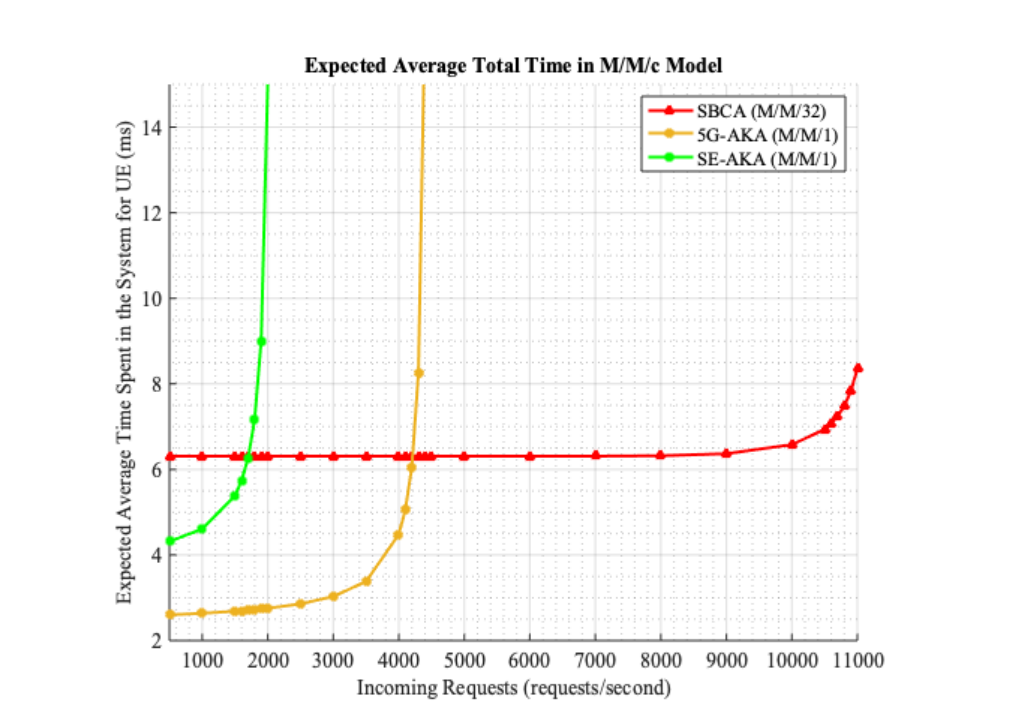
\includegraphics[width=0.8\textwidth]{images/5g-blockchain-dos.png}
    \caption{Autenticazione nelle reti 5G}
\end{figure}
\cite{5g-blockchain}